% !TEX TS-program = XeLaTeX
% use the following command:
% all document files must be coded in UTF-8
\documentclass[english]{textolivre}
% build HTML with: make4ht -e build.lua -c textolivre.cfg -x -u article "fn-in,svg,pic-align"

\journalname{Texto Livre}
\thevolume{16}
%\thenumber{1} % old template
\theyear{2023}
\receiveddate{\DTMdisplaydate{2022}{12}{21}{-1}} % YYYY MM DD
\accepteddate{\DTMdisplaydate{2023}{2}{3}{-1}}
\publisheddate{\DTMdisplaydate{2023}{4}{6}{-1}}
\corrauthor{Rafael Oliveira Vasconcelos}
\articledoi{10.1590/1983-3652.2023.42204}
%\articleid{NNNN} % if the article ID is not the last 5 numbers of its DOI, provide it using \articleid{} commmand 
% list of available sesscions in the journal: articles, dossier, reports, essays, reviews, interviews, editorial
\articlesessionname{articles}

%apagar
%\runningauthor{XXXXX e XXXXX} 
%descomentar
\runningauthor{Soares and Vasconcelos} 

%\editorname{Leonardo Araújo} % old template
\sectioneditorname{Daniervelin Pereira}
\layouteditorname{Leonardo Araújo}

\title{A distributed architecture proposal for e-voting}
\othertitle{Uma proposta de arquitetura distribuída para votação eletrônica}
% if there is a third language title, add here:
%\othertitle{Artikelvorlage zur Einreichung beim Texto Livre Journal}

%apagar
%\author[1]{Author XXXXX~\orcid{0000-0000-0000-0000}\thanks{Email: \href{mailto:XXXXX@XXXXX.com}{XXXXX@XXXXX.com}}}
%\author[2]{Author XXXXX~\orcid{0000-0000-0000-0000}\thanks{Email: \href{mailto:XXXXX@XXXXX.com}{XXXXX@XXXXX.com}}}
%\affil[1]{affiliation XXXXX}
%\affil[2]{affiliation XXXXX}
%descomentar
\author[1]{João Marcos Soares~\orcid{0000-0002-5242-3289}\thanks{Email: \href{mailto:joao.soares@dcomp.ufs.br}{joao.soares@dcomp.ufs.br}}}
\author[1]{Rafael Oliveira Vasconcelos~\orcid{0000-0001-7974-304X}\thanks{Email: \href{mailto:rafael@dcomp.ufs.br}{rafael@dcomp.ufs.br}}}
\affil[1]{Universidade Federal de Sergipe, Departamento de Computação, São Cristóvão, SE, Brasil.}

\addbibresource{article.bib}
% use biber instead of bibtex
% $ biber article

% used to create dummy text for the template file
\definecolor{dark-gray}{gray}{0.35} % color used to display dummy texts
\usepackage{lipsum}
\SetLipsumParListSurrounders{\colorlet{oldcolor}{.}\color{dark-gray}}{\color{oldcolor}}

% used here only to provide the XeLaTeX and BibTeX logos
\usepackage{hologo}

% if you use multirows in a table, include the multirow package
\usepackage{multirow}

% provides sidewaysfigure environment
\usepackage{rotating}

% CUSTOM EPIGRAPH - BEGIN 
%%% https://tex.stackexchange.com/questions/193178/specific-epigraph-style
\usepackage{epigraph}
\renewcommand\textflush{flushright}
\makeatletter
\newlength\epitextskip
\pretocmd{\@epitext}{\em}{}{}
\apptocmd{\@epitext}{\em}{}{}
\patchcmd{\epigraph}{\@epitext{#1}\\}{\@epitext{#1}\\[\epitextskip]}{}{}
\makeatother
\setlength\epigraphrule{0pt}
\setlength\epitextskip{0.5ex}
\setlength\epigraphwidth{.7\textwidth}
% CUSTOM EPIGRAPH - END

% LANGUAGE - BEGIN
% ARABIC
% for languages that use special fonts, you must provide the typeface that will be used
% \setotherlanguage{arabic}
% \newfontfamily\arabicfont[Script=Arabic]{Amiri}
% \newfontfamily\arabicfontsf[Script=Arabic]{Amiri}
% \newfontfamily\arabicfonttt[Script=Arabic]{Amiri}
%
% in the article, to add arabic text use: \textlang{arabic}{ ... }
%
% RUSSIAN
% for russian text we also need to define fonts with support for Cyrillic script
% \usepackage{fontspec}
% \setotherlanguage{russian}
% \newfontfamily\cyrillicfont{Times New Roman}
% \newfontfamily\cyrillicfontsf{Times New Roman}[Script=Cyrillic]
% \newfontfamily\cyrillicfonttt{Times New Roman}[Script=Cyrillic]
%
% in the text use \begin{russian} ... \end{russian}
% LANGUAGE - END

% EMOJIS - BEGIN
% to use emoticons in your manuscript
% https://stackoverflow.com/questions/190145/how-to-insert-emoticons-in-latex/57076064
% using font Symbola, which has full support
% the font may be downloaded at:
% https://dn-works.com/ufas/
% add to preamble:
% \newfontfamily\Symbola{Symbola}
% in the text use:
% {\Symbola }
% EMOJIS - END

% LABEL REFERENCE TO DESCRIPTIVE LIST - BEGIN
% reference itens in a descriptive list using their labels instead of numbers
% insert the code below in the preambule:
%\makeatletter
%\let\orgdescriptionlabel\descriptionlabel
%\renewcommand*{\descriptionlabel}[1]{%
%  \let\orglabel\label
%  \let\label\@gobble
%  \phantomsection
%  \edef\@currentlabel{#1\unskip}%
%  \let\label\orglabel
%  \orgdescriptionlabel{#1}%
%}
%\makeatother
%
% in your document, use as illustraded here:
%\begin{description}
%  \item[first\label{itm1}] this is only an example;
%  % ...  add more items
%\end{description}
% LABEL REFERENCE TO DESCRIPTIVE LIST - END


% add line numbers for submission
%\usepackage{lineno}
%\linenumbers

\begin{document}
\maketitle

\begin{polyabstract}

\begin{english}
\begin{abstract}

Manual voting processes have two main problems, the reliability of the result and the delay in counting the votes. To defraud the election, that is, change the amount of votes of the candidates, an attacker can replace ballots with votes for other candidates with ballots with votes for the candidate to be benefited. In this scenario, the security of the electoral process strongly depends on the control of physical access to the ballot boxes. On the other hand, electronic voting systems (e-voting) are known for their agility in counting the votes, as well as having the potential to increase the security of the electoral process. However, both solutions present challenges in relation to the transparency, security and secrecy of the vote. This work presents conceptual and technological requirements for a secure electronic election, proposes a distributed solution for electronic voting, and presents its limitations and some possibilities for future work. Finally, more studies are required to implement the solution, mainly in relation to the secrecy of the vote and incoercibility.


%Electronic voting systems present several challenges regarding security, voting secrecy and transparency. The objective of this work is to explore the necessary requirements for an electronic election, to analyze the advantages and disadvantages that a distributed architecture can add to the topic, and to propose a distributed architecture for electronic voting. The work concludes that, in a distributed architecture, the network consensus mechanism and the storage of votes are crucial points to the system design, and that technological advances are still necessary to meet all the requirements.

\keywords{Election \sep Electronic voting system \sep E-voting \sep Consensus \sep Distributed systems}
\end{abstract}
\end{english}
% if there is another abstract, insert it here using the same scheme

\begin{portuguese}
\begin{abstract}

Processos de votação manual apresentam dois principais problemas: a confiabilidade do resultado e a demora na contagem dos votos. Para fraudar a eleição, isto é, alterar a quantidade de votos dos candidatos, um atacante pode substituir cédulas com votos para outros candidatos por cédulas com votos para o candidato a ser beneficiado. Nesse cenário, a segurança do processo eleitoral depende fortemente do controle de acesso físico empregado às urnas. Por outro lado, sistemas de votação eletrônico (\textit{e-voting}) são conhecidos pela agilidade na contagem dos votos, bem como têm potencial para aumentar a segurança do processo eleitoral. Entretanto, ambas as soluções apresentam desafios em relação à transparência, segurança e sigilo do voto. Este trabalho apresenta os requisitos conceituais e tecnológicos para uma eleição eletrônica segura, propõe uma solução distribuída para votação eletrônica, apresenta suas limitações e algumas possibilidade de trabalho futuro. Por fim, são requeridos mais estudos para a implementação da solução, principalmente em relação ao sigilo do voto e incoercibilidade.

\keywords{Eleição \sep Sistema de votação eletrônico \sep E-voting \sep Consenso \sep Sistemas distribuídos}
\end{abstract}
\end{portuguese}
\end{polyabstract}

\section{Introduction}\label{sec-intro}

Proposals for electronic election systems (e-voting) seek to lower the costs of an election while maintaining integrity, security, and privacy requirements \cite{hjal}. While the efficiency and cost benefits in computerized processes are clear relative to analog processes, security care can become more complex \cite{stallings}.

The literature points to security as the primary challenge in e-voting. Works bring up the theoretical risks of e-voting compared to the risks of the traditional system \cite{lauer2004risk, Gritzalis}. Other works point out flaws in e-voting system implementations \cite{estonia, aranha}.

In this sense, the advent of cloud computing and decentralized architectures arise as an attempt to deal with the imposed security challenges, mainly related to trust in the system. With a decentralized architecture, the parties involved need to enter into an agreement on the values that will be committed. Sharing responsibilities can improve the trust in the system. To this end, it will be presented how distributed computing systems resolve conflicts and how this can be leveraged for a decentralized architecture. %Furthermore, with the emergence of blockchain technology, work has been published on the use of this technology in the context of electronic elections \cite{hjal, voas}.

The advantage of the aforementioned tool is to spread the responsibility of the system among several entities, adding redundancy. This paper seeks to present the requirements and challenges that a distributed architecture of choice must possess. Initially it was planned that the proposed format would use blockchain as a platform. However, it was realized that certain exigencies of electoral systems make the pure application of blockchain not ideal. Blockchain alone does not provide the authentication mechanisms necessary for e-voting. If the network requires participants to be identified, a central entity is needed. In addition, part of the secrecy in blockchain (more specifically in the Bitcoin network) comes from the fact that users are not authenticated and therefore can assume numerous identities.

Blockchain also does not solve the problem of secret storage of votes (which will be presented in \Cref{sec-principle-unmonitored} and discussed at the beginning of \Cref{sec-Proposal}). That is, there is no way to guarantee that the vote stored in the chain will only be available at the end of the election. Thus, the benefit of blockchain is restricted to distributed storage and immutability. For distributed storage, a traditional distributed database can solve the problem. A similar result to immutability can be achieved if the system enters into consensus on vote ciphers before disclosure (see \Cref{sec-confirmation}).

\subsection{Objectives \label{sec-objectives}}

The goal of this paper is to present a proposal for a decentralized and distributed architecture for “small electronic elections”, where the number of responsibilities of a central entity should be as few as possible. For the purposes of this research, “small electronic elections” will be understood as the internal elections of public and private institutions, student organizations, and unions.

In order to achieve the general objective, the following specific objectives have been
outlined:

\begin{itemize}
\item Present the requirements of a secure electronic election;
\item Propose a distributed election model based on the raised requirements;
\item Analyze the main challenges imposed by this model;
\item Analyze its advantages, disadvantages and viability.
\end{itemize}

\subsection{Methodology \label{sec-methodology}}

For the development of this work, exploratory research on e-voting was carried out in the literature. After that, concepts about distributed systems and cryptography were studied. Finally, an architecture based on the studied themes was proposed.

\subsection{Related work \label{sec-related}}

For the present study, articles on electronic voting were used as a basis. \textcite{Gritzalis} points out a set of principles that the development of election systems should comply with, based on constitutional principles of democratic countries. In addition, the author discusses whether e-voting should be used as a complementary means to the traditional process or conducted independently.

\textcite{lauer2004risk} lists the possible risks of e-voting, both Internet voting and the use of technology, to support the traditional election. Risks at the physical and network levels are analyzed and recommendations are made on how to mitigate these risks.

The work of \textcite{estonia} analyzes the security of Estonia's online election system, using code analysis, in-person observations, and intrusion tests on replicas of the system as a basis. The results show that there are security flaws in the architecture and that the design of electronic voting systems is difficult, as it must ensure confidence in the result while
maintaining the secrecy of the vote.

A similar work is done by \textcite{aranha}, but in the context of Brazilian elections. The authors present the electoral process in Brazil and discuss points of failure involving the electronic ballot box. It is discussed that one of the main points of failure is in the source code validation process, as it is not guaranteed that the source code that is contained in the ballot box is the same as that audited by the stakeholders. Moreover, the source code auditing process itself is limited.

The use of cloud computing for electronic elections is explored in the work of \textcite{Lekkas}. Also in this paper, the use of electronic processes in governments is reviewed, and a set of threats are listed, such as malicious code on the client, message interception, and
their respective security measures.

%In the context of cloud computing for elections, a few papers study the use of blockchain. \textcite{voas} presents blockchain as a possible solution for e-voting. The authors argue that voters can send secret ballots from their own smartphone and that the blockchain system would provide authentication. The results could not be changed due to blockchain's immutability property and therefore the votes would be secure. The article is introductory and does not clearly present how the technology can be used, draw parallels with the requirements of an election, or discuss possible flaws. The authors cite examples of election events that have used blockchain in Russia, South Korea, and Sierra Leone, but the sources do not indicate publicly available articles that describe the election process in each.

%\textcite{hjal} proposes an election system using a permissioned blockchain network, that is, a network that only authenticated users can use. While highlighting that one of the requirements of the solution is intraceability, the paper does not make explicit how the vote is stored on the network, other than making it clear that the voter can in the future verify his or her own vote with a generated ID.

%\textcite{Hardwick} also explores the use of blockchain for the storage of votes in an e-voting scheme. For the authors, blockchain's features of anonymity, transparency, and security fit the requirements of an election. In this scheme, although the goal is to create as distributed a network as possible, there is a central authority responsible for managing the identities of voters. Furthermore, to minimize the effects of coercibility (The principle of incoercibility will be discussed in \Cref{sec-principle-Incoherence}) the author proposes that the vote is tied to the voter until the end of the election and that this vote can be freely modified. Thus, if the voter is coerced at the moment of casting the vote, he will be able to change it in the future at a more favorable moment.


\section{Background \label{sec-background}}

In this section, the issues that serve as a basis for the paper will be presented. \Cref{sec-requirements} presents the principles necessary for the development of a secure electronic election system. \Cref{sec-consensus} presents the concept of distributed systems and consensus algorithms. \Cref{sec-time} introduces concepts of time-based encryption. %\Cref{sec-moderately} shows what moderately hard functions are and their applications. \Cref{sec-time} introduces concepts of time-based encryption.

\subsection{Requirements for a secure electronic election \label{sec-requirements}}

The first step in building the architecture of a secure election system is to define the requirements for it to be considered secure and effective. Several papers in the literature \cite{Lekkas, Sampigethaya, Hardwick} use the work of \textcite{Gritzalis} as a reference for requirements’ mapping.

\textcite{Gritzalis} defines a series of design fundamentals that should be followed when developing e-voting systems. They derive from from constitutional principles in democratic countries. These principles sometimes complement and sometimes contradict each other. It is therefore impossible to design a system (whether traditional or electronic) that completely satisfies all of them. The principles are listed below.

\subsubsection{Principle of isomorphism to the traditional process \label{sec-Principle-Isomorphism}}

The electronic electoral process must guarantee the characteristics of the traditional universal suffrage electoral process. For this, the following premises are defined:

\begin{enumerate}


\item Every voter has the right to participate in the electoral process;

\item The definition of the individual as a voter must be found and controlled by law;

\item The technology to cast the vote must be accessible to all voters;

\item E-voting should be considered an alternative means of voting;

\item The democratic principle (i.e, every voter has the right to participate in the electoral process) leads to the need for adequate public infrastructure (free internet points, etc).

%%\end{itemize}
\end{enumerate}

These definitions were made for national elections. For more restricted electoral processes, such as those at a university, the law mentioned in item 2 of the above premises can be replaced by internal regulations. The important thing is that the rules defining who can vote exist. Consequently, in item 5, the important thing is to ensure that voters have access to the necessary infrastructure to exercise their political will. It is also through this principle that it is necessary for the voting system to ensure that the voter is authenticated to vote.

\subsubsection{Principle of voting eligibility}

Voters must be able to register and authenticate themselves in order to cast their vote. This principle does not conflict with the previous principle, since in order to be considered a voter, the individual must meet the criteria laid out in the rules defining who can vote in those elections, and it also prevents a voter from being able to vote more than once.

\subsubsection{Principle of incoherence \label{sec-principle-Incoherence}}

It must be guaranteed that the vote cannot be bought, and that the voter cannot be extorted. This principle can only be achieved if the voter is unable to prove that he or she voted for a particular proposal. In addition to the technical requirements for this, the public voting structure (e.g. polling booth) must ensure that the person cannot be coerced outside the system.

\subsubsection{Principle of freedom of decision \label{sec-principle-freedom}}

The voter's freedom of decision can be violated if any party or candidate advertisement is broadcast during the casting of the vote. In the traditional electoral process, no advertising is permitted at the polling station. Similarly, in an electronic voting process, no election advertising should be permitted on the voting site or generally on the system interface.


\subsubsection{Principle of the invalid voting option}

The voter should have the freedom of preference preserved. This means that if none of the available options appeals to him, he should be able to cast an invalid (null) vote.

\subsubsection{Principle of equality among candidates}

The interface of the system should not favor or disadvantage candidates. This principle is similar to the principle of Freedom of Decision, but with a focus on candidates. The positioning of ballots in a traditional election and the display of candidates on a computer screen should provide equality among candidates.

Moreover, all candidates should have equal access to the transparency of the election. That is, they should all have access to the same tools and information to check and audit the correct functioning of the election process.

\subsubsection{Principle of equality among voters (One voter, one vote) \label{sec-one-vote}}

The principle of Equality Among Voters states that all votes should have the same value. From this premise, three pieces of information are derived. The first is that there should be no system of weights where one individual's vote is worth more than another. The second is that a voter can cast one, and only one, vote.
Finally, \textcite{Phillips} argue that in the context of electronic voting, access to and familiarity with the technology may give a certain group of voters an advantage when casting a vote. Also, for this reason, access to the tools to cast the vote should be universal, as discussed in the Isomorphism principle (\Cref{sec-Principle-Isomorphism}). On the other hand, for people who for whatever physical reason (comorbidity, geographical distance) cannot attend a traditional polling place, the e-voting system can help make the principle of Equality Among Voters true.

As aforementioned in \Cref{sec-requirements}, \textcite{Gritzalis} claims that it is apparently impossible to guarantee the principle of “One voter, One vote”. However, one possibility to guarantee such requirement is ensuring the e-voting system to register that the voter cast the vote. Thus, the system can prevent a voter from casting multiple votes. On the other hand, concerning impaired people or people unfamiliar with the technology, the organizing institution may have some campaigns or initiatives to assist those people.

\subsubsection{Principle of secrecy \label{sec-Secrecy}}

This principle is linked to the principle of incoherence and freedom of decision (\Cref{sec-principle-freedom}). Secrecy is a necessary requirement to ensure free political decision. Once cast, the vote should be irreversible and not even the voter himself should be able to recover his decision.

In traditional electoral systems, secrecy is guaranteed by physical barriers, however, \textcite{Gritzalis} believes that in e-voting systems secrecy can be compromised, and that the following requirements must be explicitly met:

\begin{itemize}
\item Secrecy of the vote must be guaranteed in the casting, in the transport (in this case by network), in the reception and counting;

\item None of the actors involved (organizers, candidates, and voters) should be able to make the connection between a voter and a vote;

\item There should be a well-defined separation between the registration and authentication processes and the vote-casting and collection processes;

\item No voter should be able to prove that he or she voted for a particular candidate.

\end{itemize}

It is pertinent to point out that in any remote voting system, there is no guarantee that the individual will not be coerced at the time of casting the vote, for this reason, when designing e-voting systems, external protective measures should be discussed, such as voting booths \cite{Gritzalis}. As mentioned, these principles are contradictory since some measures create a conflict with the Equality principle, which may exclude those people who were unable to move to the voting center. Thus, the organizer should provide some assistance program for those with special needs, as stated in \Cref{sec-one-vote}.

\subsubsection{Principle of unmonitored voting \label{sec-principle-unmonitored}}

During the electoral process, third parties cannot monitor voting. In traditional elections, this principle is enforced with measures that ensure that the ballot box is only opened at the time of vote counting. In an electronic voting context, it must be ensured that the computed votes can only be read after a certain moment, which indicates the end of the reception of votes. If this does not occur, the entity storing the votes may perform monitoring.

\subsubsection{Principle of transparency \label{sec-Transparency}}

The e-voting election process should be as transparent as possible and the faith in the system as low as possible. That is, in an ideal situation, all actors involved (organizers, candidates, and voters) should be able to understand how the election takes place. \textcite{Gritzalis} emphasizes that faith in the system is an inherent factor in electronic voting, since an ordinary citizen has no knowledge about how computer systems work. Although the common voter does not know how computer systems work, the e-voting system should be audited by reliable third parties, as it happens in the Brazilian electoral system, for instance.

Therefore, it is important that the electronic electoral system be transparent and that the processes involved be explained, even if in a high-level language. This characteristic must accompany the system itself.

\subsubsection{Principle of verifiability and accountability \label{sec-Accountability}}

Verifiability is the ability of voters, candidates, organizers, and independent observers to verify that the electoral process occurs in the correct manner. Accountability relates to the system's ability to produce logs and monitoring of all election operations, so that any individual can search for inconsistencies.

However, the voter's ability to verify that his or her vote has been counted and counted completely contradicts the principle of Secrecy (\Cref{sec-Secrecy}) and Incoherency (\Cref{sec-principle-Incoherence}). In general, electoral systems (both traditional and electronic) make a trade off and give up some of the verifiability and accountability to maintain the secrecy of the vote.

\subsubsection{Principle of simplicity \label{sec-Simplicity}}

The principle of Simplicity states that the system should be as simple as possible. Simplicity, then, coupled with the principle of Transparency (\Cref{sec-Transparency}), seeks to ensure that the system is user-friendly, that is, simple, accessible, and understandable to the user. However, due to principles such as Security and Reliability (\Cref{sec-Reliability-sec}), the system's source code is unlikely to be simple, given the inherent complexity of the system.

\subsubsection{Principle of reliability and security \label{sec-Reliability-sec}}

This principle permeates several other principles mentioned above. Reliability means that the election result is truly a reflection of the will of the electorate, so the system must ensure that the election result is in accordance with the votes cast and that these have not been modified and are true to what the voters want. No votes cast should be allowed to be excluded, and invalid votes should be counted, in accordance with the Invalid Vote Option principle. Just as in Secrecy (\Cref{sec-Secrecy}), Reliability and Security should also be enforced in all stages of the voting process (i.e., casting, transportation, reception and counting).

Security refers to ensuring the secrecy, integrity, and availability of the system. The process of registration and authentication of actors must be done in a secure manner and the system must be available and protected against denial-of-service attacks, intentional or not, since the unavailability of the system hurts the right of the voter to cast his vote.

In a sense, Security counteracts the Simplicity principle since security processes inevitably end up increasing the complexity of the system.

Based on the principles of Reliability, Security (\Cref{sec-Reliability-sec}), Verifiability and Accountability (\Cref{sec-Accountability}), \textcite{Gritzalis} proposes the following requirements:

\begin{itemize}

\item There must be hardware and software certification processes;


\item All infrastructure as well as system functionality should be verifiable and comply with Kerckhoff's requirement in order to remain secure even if it is open-source \cite{katz2020introduction, Kerckhoffs};

\item All operations should be monitored and generate system logs, except those that might break the secrecy of the vote;


\item The infrastructure should be open for inspection by authorized agents;

\item Voters and candidates should be assured that there were no malpractices during the process.

\end{itemize}

\subsection{Consensus in distributed systems \label{sec-consensus}}

A distributed system is a collection of independent computers that cooperate to solve a problem that cannot be solved individually \cite{Kshemkalyani}. More precisely, the entities of a distributed system have the following characteristics:

\begin{itemize}

\item Independent physical clocks: The clocks in the network are not necessarily synchronized; this becomes an obstacle for managing the order of the exchanged messages. This problem was the motivation for \textcite{Lamport} work that gave rise to logical time theory;

\item Independent Memories: Entities do not share memory, i.e., all communication depends on messages;

\item Autonomy and heterogeneity: Processes have different speeds and can run on different operating systems, with different implementations.

\end{itemize}

Since the communication medium is the most important aspect of the network, it is necessary to classify the errors that can occur during message transmission. The worst type of error in this context is the byzantine failure, defined by \textcite{lamport2019byzantine}. In this fault, nodes can show any arbitrary error in the message exchange, including purposeful alteration of the content. In a variation of this problem, the Byzantine failure with authentication, the same errors can occur, but the messages can be verified through signatures.


One of the major problems in distributed systems is the consensus among the nodes. That is, how a network of nodes agrees on a certain value. In the context of Byzantine failures, the best known proposed algorithm is Practical Byzantine Fault Tolerance, or PBFT, proposed by \textcite{liskov}. In this algorithm, it is possible to guarantee consensus on up to $\frac{n-3}{3}$ malicious nodes, where $n$ is the total number of nodes. Another consensus algorithm proposed later is Proof-of-Work. %, which will be worked on in more detail in \Cref{sec-blockchain}.

Blockchain is an append-only data structure, meaning that the only modification allowed is the addition of more data. Data is entered in blocks, so that each block has a hash of the previous block \cite{nakamoto}.

Since the network has no central entity, the nodes need to decide together which one will add the next block to the chain. The most intuitive solution is a lottery. However, this form of random selection is susceptible to attacks and requires some node to assume a centralizing role \cite{zheng}.

The Proof-of-work algorithm \cite{dwork} is then used, where nodes need to prove that they have performed certain work to generate a new block and add it to the network. For this algorithm, work can also be interpreted as time expenditure, expressed in CPU cycles. In later work, the idea of the algorithm is extended so that the node can spend other resources, such as space or digital coins \cite{dziembowski2015proofs, gavzi2019proof}. 

%\subsection{Blockchain and Proof-of-Work \label{sec-blockchain}}

%Blockchain is an append-only data structure, meaning that the only modification allowed is the addition of more data. Data is entered in blocks, so that each block has a hash of the previous block \cite{nakamoto}.

%Since the network has no central entity, the nodes need to decide together which one will add the next block to the chain. The most intuitive solution is a lottery. However, this form of random selection is susceptible to attacks and requires some node to assume a centralizing role \cite{zheng}.

%The Proof-of-work algorithm \cite{dwork} is then used, where nodes need to prove that they have performed certain work to generate a new block and add it to the network. For this algorithm, work can also be interpreted as time expenditure, expressed in CPU cycles. In later work, the idea of the algorithm is extended so that the node can spend other resources, such as space or digital coins \cite{dziembowski2015proofs} \cite{gavzi2019proof}. 

%For bitcoin, it is a network requirement that block hashes must begin with a certain number of zeros. This number of zeros at the beginning of the hash is called the target. For this, in addition to the transaction history, the blocks need to have an element called a nonce. The job that the node must do is to find a nonce that, added to the the other data in the block, generates a hash with the predefined number of zeros at the beginning. The work to be performed is exponentially proportional to the goal, and in the Bitcoin network the goal increases over time \cite{nakamoto}.

%\subsection{Moderately Hard Functions \label{sec-moderately}}

%Nakamoto's article cites the work of \textcite{hashcash}, who in turn cites \textcite{dwork}, as the origin for Proof-of-work. In the latter article, the authors discuss a way to combat spam by using a rate for sending e-mails that does not disrupt the user experience but makes it difficult to send mass messages. The solution was to require the computer to prove that it did work by performing a function that is not trivial, but also not impossible, i.e., a Proof-of-work.

%Authors \textcite{dwork} called these functions that are non-trivial but at the same time not intractable moderately hard functions, proposing a new field of study and suggesting that more research in the area be conducted. Examples of applications that may benefit from the advancement of this area are temporary resource locking and as proof of effort accomplishment, as discussed in \Cref{sec-blockchain}. Naor (2003) proposes that moderately hard functions can be used as a form of time-based encryption using essentially sequential functions, i.e., functions that cannot be parallelized. Thus, the time estimate for breaking a problem is approximately the same regardless of the computational power of the agent.

%\subsection{Asymmetric Cryptography \label{sec-asymmetric}}

%In 1976, the work of \textcite{diffie} was the first to publicly introduce the concept of asymmetric cryptography. In this form of cryptography, there is one key to do the encryption and a different but related key to do the decryption. Furthermore, it is computationally impractical to determine the decryption key using the encryption key.

%In a public-key system, as in the RSA algorithm \cite{rsa}, if one of the keys is used for encryption, the other is used for decryption, which generates two major advantages: the first is that sending encrypted messages without having to share a secret; the second is that it becomes possible to sign messages to guarantee their origin and authenticity.
%The step-by-step basic operation is as follows \cite{stallings}:

%\begin{itemize}

%\item Each user generates a key pair;

%\item Each user makes one of the keys available to anyone (public key) and keeps the other key secret (private key);

%\item If Bob wants to send a confidential message to Alice, Bob encrypts the message with Alice's public key;
%\item When Alice receives the encrypted message, she decrypts it using her private key. since only she has the private key, only she can decrypt it;

%\item If Bob wants to send a message to Alice, so Alice is sure Bob is the author, he encrypts the message using his private key;

%\item When Alice receives the cipher, she decrypts it using Bob's public key. That is, only Bob could have written the message.

%\end{itemize}


%\autoref{encriptacao-chave-publica} represents this process. In image (a), Bob encrypts the text $X$ with Alice's public key $PU_{a}$ and an asymmetric encryption algorithm $E$, generating the cipher $Y$ , such that$Y = E(X, PU_{a})$. Alice decrypts $Y$ with her private key $PR_{a}$ and a decryption algorithm $D$, such that $D(Y, PR_{a}) = X$. In image (b), Bob encrypts the text $X$ with Alice's private key $PR_{b}$ and an asymmetric encryption algorithm $E$, generating the cipher $Y$ , such that $Y = E(X, PR_{b})$. Alice decrypts $Y$  with Bob's public key $PU_{b}$ and a decryption algorithm $D$, such that $D(Y, PU_{b}) = X$.
%Traditionally, this system can be used to exchange secret messages and to generate digital certificates.

%\begin{figure}[htb]
%\centering
%  \caption{\label{fig_grafico}Asymmetric encryption example.}
%  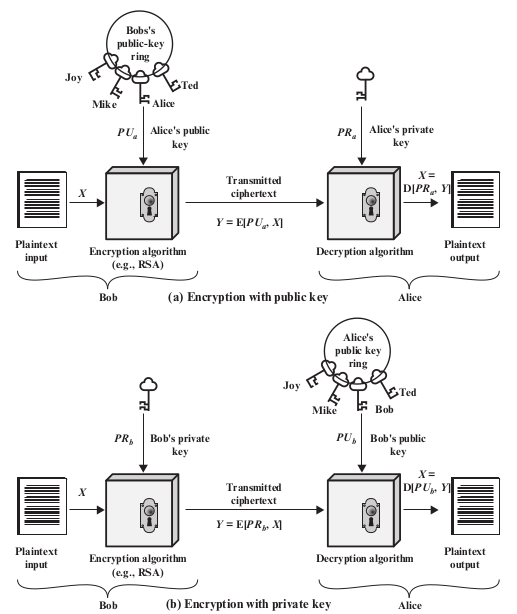
\includegraphics[scale=0.75]{imagens/private-public.png}
%  \label{encriptacao-chave-publica}
%  \source{\cite{stallings}.}
%\end{figure}


\subsection{Time-Based encryption \label{sec-time}}

An interesting problem in the area of cryptography is the study of how to create a way to block access to a piece of information for a period of time, and after that period the information becomes available without requiring an action from the person who blocked it. The problem is also sometimes described as “sending a message to the future”.

Some approaches have been proposed to deal with this problem. One line of research proposes models that assume a trusted third party is responsible for releasing decryption keys at the correct time \cite{rivest1996time, boneh2005hierarchical, palestrinha}. Another line of research uses the idea that the receiver of the message needs to solve an expressive, but not impossible, computational problem to unravel the cipher \cite{timedcommitments, unruh2015revocable}. The difficulty of the problem defines the approximate time for the cipher to be revealed, and the problems themselves are chosen so that the computational effort cannot be parallelized.


\textcite{Liu} defines that to have complete time-based encryption, the three criteria must be met simultaneously:

\begin{itemize}

\item \textbf{Non-interactivity}: The sender of the cipher is not needed for decryption;
\item \textbf{Independence}: There should be no dependency on a trusted third party. That is, the issuer does not need to depend on a trusted third party to store the decryption keys until the time of the cipher opening arrives.
\item \textbf{Resource savings}: Interested parties in revealing the cipher should not be forced to spend computational resources for this purpose. This means that a receiver should only wait until the planned release time of the cipher to discover the message, and all stakeholders should discover the message at approximately the same time regardless of computational power.

\end{itemize}

\textcite{Liu} proposes a solution that theoretically meets all three requirements. The authors introduce the idea of a reference computational clock, based on the state of a public, constantly iterative distributed computation. As an instance of this clock, the authors use the Bitcoin network. Added with the reference clock, a witness encryption scheme is used \cite{garg2013witness}


\section{Proposal \label{sec-Proposal}}

Following the principles proposed by \textcite{Gritzalis} described in \Cref{sec-requirements}, this section presents a distributed architecture for e-voting. The goal of this architecture is that the election participants depend as little as possible on a central authority to conduct the election. The election should be managed in a distributed manner, even among adversarial parties, as proposed in \Cref{proposal}:

\begin{table}[htpb]
\centering
\small
\begin{threeparttable}
  \caption{Transfer of responsibility in a decentralized model}
  \label{proposal}
  \begin{tabular}{lll}
  \toprule
   Action & Responsibility in centralized model & Responsibility in decentralized model \\
  \midrule 
   Manage Voters & Central Authority & Central Authority \\
   Managing Candidates & Central Authority & Central Authority, candidates, observers \\
   Casting Votes & Voter & Voter \\
   Storing Votes & Central Authority & Candidates, observers \\
   Perform counting & Central Authority & Candidates, observers \\
   Auditing the system & Voters, candidates, observers & Voters, candidates, observers \\
  \bottomrule
\end{tabular}%
\source{Author.}
\end{threeparttable}
\end{table}

In this work, three types of roles played by the network nodes are defined:

\textbf{Voters}: these are the nodes responsible for casting votes. Following the Isomorphism Principle (\Cref{sec-Principle-Isomorphism}), voters must be authenticated to cast the vote. It should be possible for the voter to ensure that his vote has been computed, but it should not be possible for him to generate evidence of the content of his own vote (Principles of Verifiability and Incoherence, respectively). At the end of the election, voters should be able to verify and audit the vote count.

\textbf{Hosts}: are the nodes that store the votes. Candidates (or parties) must play the role of hosts. Assuming that an election has at least two candidates, then there must be at least two hosts. Other individuals, entities or observers with an interest in being hosts can also play the role.

\textbf{Certificate Authority}: Node responsible only for issuing and verifying digital certificates. It is the central entity (physically it can be distributed) with reduced power when it comes to issuing and counting votes. It is an identity and authorization query node for the other nodes. Before the election, it is necessary that all future participants (voters, candidates, other interested parties) have public keys registered with the Certificate Authority. Throughout the paper it will be abbreviated to CA.

Two major challenges arise with this model:

\begin{enumerate}

\item How should the hosts come to consensus on vote storage?

\item What mechanism will prevent hosts from reading votes before the voting is over?

\end{enumerate}

The first problem can be addressed using the literature on consensus in distributed systems, inevitably capturing its advantages and disadvantages. Importantly, in this model, although the vote is secret, the actors involved must be properly authenticated, even if there are operations that protect the user's identity, complete anonymity is undesirable for the solution, because it would break the principle of Equality – i.e., “One voter, one vote” –  among voters once the system wouldn't even know if a particular individual casted a vote. As a consequence, one might vote more than once, breaking the principle of Equality (\Cref{sec-one-vote}). However, complete anonymity wouldn't impose that votes have different weights. This means that the messages exchanged must be authenticated in one way or another. That is, among the possible failure models in distributed systems, the goal is for the proposed model to be Byzantine failure tolerable with authentication.

The second problem is more complex. In other contexts, when an actor needs to store information in an untrusted repository, that information is encrypted; to decrypt it, an action by the actor himself or another actor authorized by him is required. The problem arises in the context of an election, when at a certain point in the electoral process, the vote needs to be disassociated from the voter. In this case, it is necessary that the encryption protecting the vote be broken only in the counting and result stage, without action from the actor that encrypted it, which in this context is the voter. Ideally, this encryption system needs to fulfill three properties simultaneously:

\begin{itemize}

\item The voter does not need to be present for decryption;
\item The system cannot depend on a third party who will keep the decryption keys;
\item The parties interested in decrypting the cipher cannot have a significant advantage over each other according to their computing power. That is, all parties must be able to decrypt the vote at approximately the same time and never before the start of the vote counting and result stage.

\end{itemize}

Therefore, this encryption needs to be time-based. For the proposed model, it is defined that the encryption mechanism is based on the work of \textcite{Liu}, because the three properties above are analogous to the properties of his proposal. However, other approaches are also valid such as a time-lock encryption where the central authority keeps the secret decryption key until the end of the voting process. The main drawback of such approach is that the CA is a central actor that hold all the secret decryption keys and may be attacked (e.g., it may suffer a Denial of Service attack or have all the decryption keys leaked). % An alternative based on moderately hard functions will also be presented (see \Cref{sec-moderately}).

\subsection{Rules, constraints, and notations \label{sec-rules}}

To serve as a basis for building and understanding the proposed model, it is necessary to define the set of rules and assumptions of the proposal:

\begin{itemize}

\item The system consists of a distributed set of nodes;

\item The notation for the asymmetric key pair of a node $n$ is $(PK_{n}, PR_{n})$, where $PK_{n}$ is the public key and $PR_{n}$ is the private key. The notation $E(m, k) = c$ means that message $m$ is encrypted with key $k$ and generates a cipher $c$. The notation $D(c, k) = m$ means that cipher $c$ is decrypted with key $k$ and generates message $m$;

\item Nodes can participate in an event called Election. During an Election, the following rules exist:

\begin{itemize}

\item An election is composed of a question $q$, which can be answered with a proposal $p$, which may be a blank or null vote. The set of proposals is $P$;

\item Each host can issue only one proposal $p$;

\item Each voter may cast only one vote $v$, to show support for only one proposal of any kind. The notation for extracting a proposal from a vote is $fv(v) = p_{n}$. The set of votes computed from an election is $V$ and $V$* is the set of valid votes (i.e., blank and null votes aren't considered valid votes) computed from the same election;

\item The number of candidates must be less than or equal to the total number of hosts;

\item The number of candidates must be greater than 1.

\end{itemize}

\item Nodes are required to perform the voting steps over a computer network (i.e., online);

\item The nodes use the NTP (Network Time Protocol) to synchronize the clocks;

\item Message exchanges between nodes are done with end-to-end encryption.

\end{itemize}

\subsection{Phase one: election setup \label{sec-phase-one}}


An election is commonly divided into three stages (\Cref{fig_grafico}): a preparation, where the characteristics of the election are defined; the vote casting period, which occurs sometime after the close of the first stage; the vote counting, which can occur immediately after the election ends. The divisions between these time periods will be called $t_{0}$, $t_{1}$, $t_{2}$.

\begin{figure}[htb]
\centering
\begin{minipage}{.8\textwidth}
   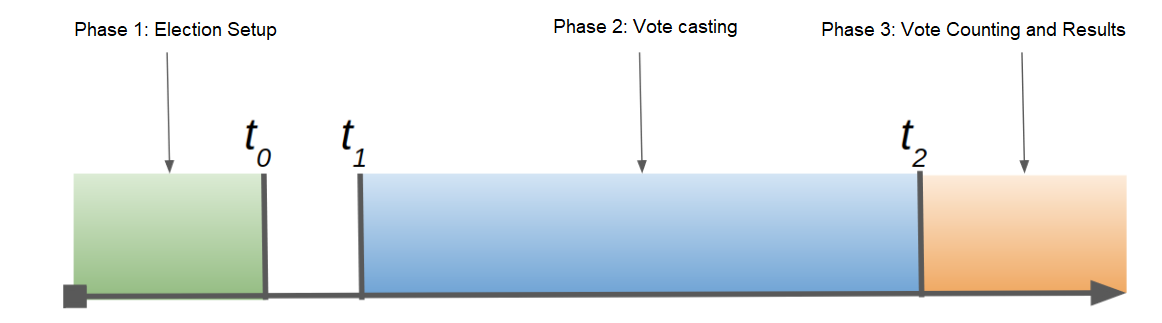
\includegraphics[width=\textwidth]{imagens/fig-001.png}
   \caption{Election timeline.}\label{fig_grafico}
   \source{Author.}
\end{minipage}
\end{figure}


\textbf{Step 1 (Creating the election)}: An election is created from any node in the network. The election is a 6-tuple $e$:

\[
 e=\langle q, t_{0}, t_{1}, t_{2}, f, bs \rangle
\]

The first element is the question $q$. The question q represents the question that is to be answered by the election. Examples of questions are \textit{"Which party should run the student center?"} or \textit{"Should the United Kingdom leave the European Union?"}. The second is a future timestamp $t_{0}$, which indicates a maximum deadline for nodes to submit proposals. The third is a future timestamp $t_{1}$, which indicates the start of receiving votes. The fourth is another future timestamp $t_{2}$, indicating a maximum time limit for votes to be received. Although this is a distributed system, it is not necessary to use a \posscite{Lamport}, logical clock scheme because there is a tolerable clock synchronization difference such that using NTP is sufficient. The fifth element is the function $fw:V\longrightarrow P$ that defines the winning proposal based on the set of votes. For example, let $A$ be the set of votes on a proposal $p_{n}$. That is, $v \in A$ if $fv(v) = p_{n}$. If it is decided that the winning proposal is the one with a simple majority, then $fw(V) = p_{n}$, if $|A| > 0.5|V|$. The sixth element is a parameter $bs \in \mathbb{N}$ e $bs < |E|$, where $E$ is the set of voters, which indicates the size of the disclosure blocks. Hosts must disclose votes in groups to balance secrecy and verifiability. This process is detailed in \Cref{sec-confirmation}.

The initiating node must make $e$ public to the other nodes. To ensure the authenticity of the proposal, the node must sign the message.

\textbf{Step 2 (Proposal and Host Registration)}: Upon learning of an election $e$, any node $n$ can issue a proposal and become a candidate before time $t_{0}$. To do this, in addition to proposition $p_{n}$, it must define a host address $h_{n}$ from which it will receive and store votes. The candidate must then make public $p_{n}$ and $h_{n}$ and sign the message containing both values to guarantee its origin. Others interested in maintaining a storage node (i.e., host) can also perform the same process, but without generating the proposal.



\begin{figure}[htb]
\centering
\begin{minipage}{.8\textwidth}
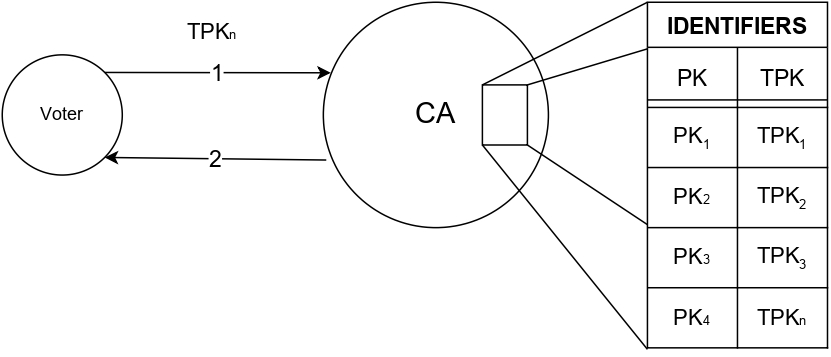
\includegraphics[width=\textwidth]{imagens/fig-002.png}
\caption{Step 1: Sending the temporary keys to the CA.}\label{fase2etapa1}
\source{Author.}
\end{minipage}
\end{figure}


\subsection{Phase two: voting and storing \label{sec-phase-two}}

\textbf{Step 1 (ID Generation):} With the arrival of $t_{0}$, the first phase is closed and, at this point, a voter node $n$ has the information about the election with a copy of the structure e, a list of proposals $p_{1}, p_{2} ... p_{n}$ and a list of host addresses $h_{1}, h_{1} ... h_{k}$, so that $n \le k$. The voter then needs to generate a temporary ID that meets the following requirements:

\begin{itemize}
\item it must be possible for the CA to verify that the ID was generated by a valid voter and that this ID is the only one generated by that voter for that election. That is, each voter must have one and only one ID;
    
\item It should not be possible for other participants in the election to associate an ID with a voter;

\item Anyone should be able to verify whether an ID is valid for that election.

\end{itemize}

To comply with the third requirement, the voter must generate a pair of keys $I = (TPK_{n}, TPR_{n})$ that will serve as a temporary identification and register it with the CA $TPK_{n}$, (message 1 in \Cref{fase2etapa1}). The CA must check if any identification of that voter already exists for that election and respond to the voter if the registration was done successfully (message 2 in \Cref{fase2etapa1}).

\begin{figure}[htb]
\centering
\begin{minipage}{.8\textwidth}
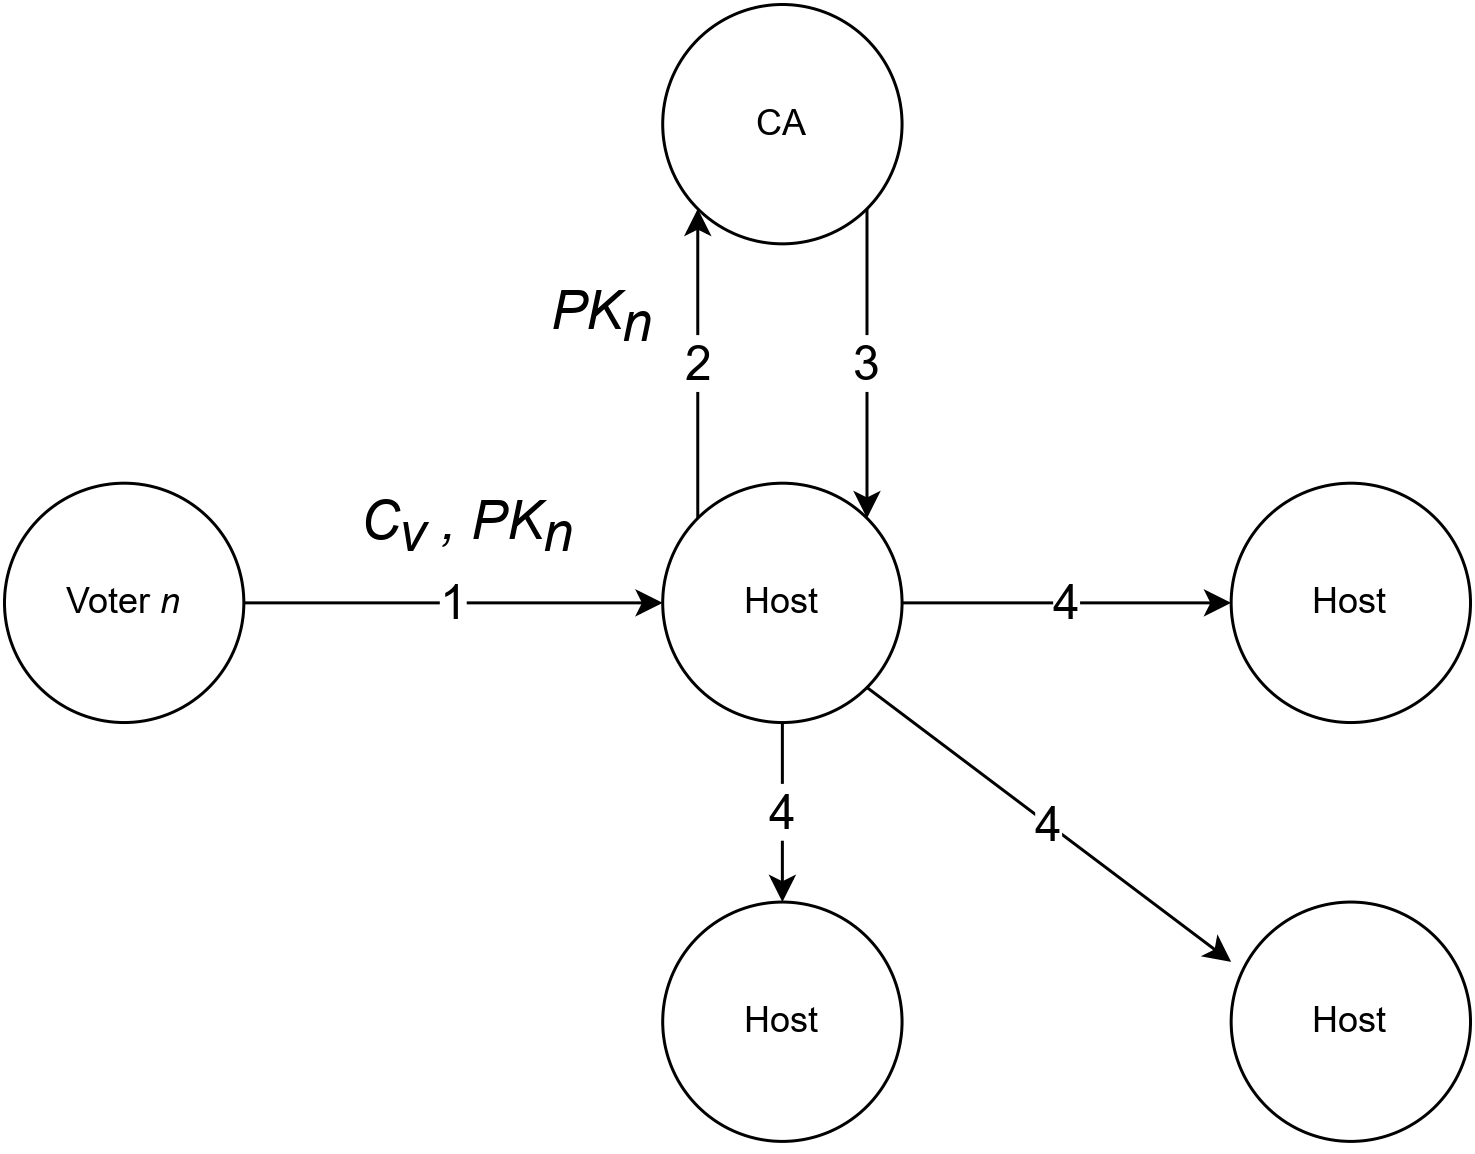
\includegraphics[width=\textwidth]{imagens/fig-003.png}
\caption{Step 2: message exchange sequence for vote submission.}\label{fase2etapa2}
\source{Author.}
\end{minipage}
\end{figure}


\textbf{Step 2 (Sending the vote):} After time $t_{1}$, the voter can cast his vote $v$, encrypted, and following the requirements described at the beginning of this section. To do so, he must use a time-based encryption scheme, grounded in the work of \textcite{Liu}. The cipher $c_{v}$ represents the cipher of the vote after encryption.

The voter must send $c_{v}$, signed with $I$, to a host $h_{i}$ any of the election (message 1 in \Cref{fase2etapa2}). The host should check with CA whether the public key of $I$ is valid (message 2 in \Cref{fase2etapa2}). If it is not, the message should be ignored. If it is valid, the host must share the signed cipher $c_{v}$ with all other hosts, using a consensus algorithm (message 4 in \Cref{fase2etapa2}).

\subsubsection{Consensus}

As discussed at the beginning of this section, the consensus between hosts needs to be Byzantine fault tolerant with authentication. In addition, the requirements that the algorithm must meet in the context of distributed election will be defined.

The first requirement is that if the voter sends a signed cipher $c_{v}$ to a host $h_{i}$, it must receive confirmation of receipt by another host $h_{j, j \neq i}$. This is done to assure the voter that there has been a consensus and that the message has been distributed. The second requirement is that each time a host receives a signed cipher $c_{v}$, it must verify the validity of the signature's public key with CA. In addition, the host needs to verify whether this is the first vote of the voter or if there is already another vote agreed upon consensus. This requirement serves as host verification that the message originated from a valid voter. Any consensus algorithm that meets these requirements, for example PBFT, can be used in this phase.



\subsubsection{Confirmation and display of votes \label{sec-confirmation}}

After the consensus is performed, some host $h_{j \neq i}$ must send a confirmation of receipt to the voter. When the voter receives the confirmation from a host $h_{j \neq i}$, the vote submission operation is completed.

After a certain $bs$ amount of vote ciphers are received, the hosts must publicly disclose these ciphers in a table, along with the accompanying $TPK$ public key values. The key and cipher values cannot be linked with each other and therefore the order of the columns must be random (see \Cref{randomizacao}). The disclosure of these tables in this way is done for two reasons that seek to meet the verifiability principle. The first is that the ciphers must be public before they are opened. Moments before the cipher is decrypted, everyone will have a copy of the vote set. The second reason is that if the cipher set is accompanied by a set of temporary public keys, even if in random order, it is possible for anyone to check with the CA whether the keys are valid.

\subsubsection{Phase summary}

The complete sequence of actions for this phase is:

\begin{enumerate}
    \item  The voter generates $I = (TPK_{n}, TPR_{n})$;
\item The voter sends a registration message from $I$ to CA;
\item CA sends a confirmation message to the voter;
\item The voter sends the $c_{v}$ message, signed with $I$ to a host $h_{i}$;
\item The host checks with CA whether $TPK_{n}$ belongs to a valid identity;
\item If the answer is positive, the host sends in groupcast $c_{v}$ to the other hosts;

\item All other hosts $h_{j \neq i}$ perform the verification of $TPK_{n}$ with CA;

\item At least one host $h_{j \neq i}$ sends the acknowledgement to the voter and to $h_{i}$;

\item The voter waits to receive confirmation from at least one host by a fixed timeout or as a parameter specified at election creation. If this does not occur, the voter repeats the send to a host $h_{j \neq i}$

\item $h_{i}$ waits to receive confirmation from at least one $h_{j \neq i}$ by the specified timeout to accept the vote. If this does not occur, the vote is discarded.

\item For any host, after a number of $bs$ votes accepted, a table is published with a column of $TPK$ and a column of $c_{v}$, both in random order.

\end{enumerate}

\begin{figure}[htb]
\centering
\begin{minipage}{.8\textwidth}
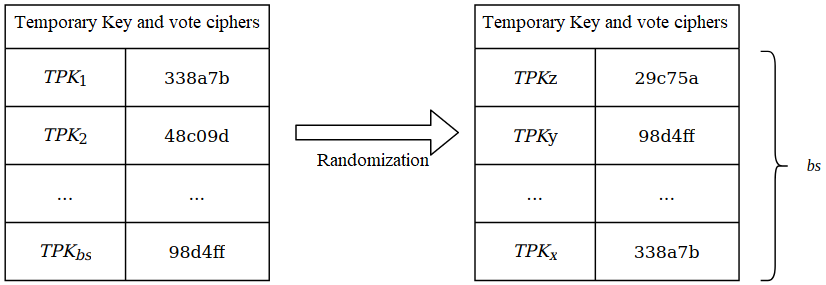
\includegraphics[width=\textwidth]{imagens/fig-004.png}
\caption{Phase 2:  Randomization of the voting cipher table}\label{randomizacao}
\source{Author.}
\end{minipage}
\end{figure}

\subsection{Phase three: counting the votes \label{sec-phase-three}}

After timestamp $t_{2}$ arrives, vote collection must be terminated. At this point, each host has already released tables with the consensus vote figures, and all interested parties can access them. If $t_{2}$ arrives and the number of votes is less than $bs$, the hosts release a smaller table. Following what was proposed at the beginning of this section, after time $t_{2}$, the ciphers are undone, and the winning proposal can be extracted from the set of votes using the $fw:V\longrightarrow P$ function defined at the time of election creation. Therefore, the counting is not the responsibility of only one actor, the verification and counting of the votes can and should be performed by multiple entities.

%\subsection{Alternative for vote encryption \label{sec-alternative}}

%In this section, an alternative to encrypting the vote is proposed using asymmetric encryption and moderately hard functions.

%Suppose Alice needs to send a message to Bob and Carlos, but the message must be opened a little after time $t$, but never before. Bob and Carlos are adversaries, so one doesn't want the other to see the messages before $t$. Also, Alice should not be needed to decrypt the messages.

%Alice could use Timed Commitments \cite{timedcommitments} to encrypt the message and send it to both of them. The problem is solved for only one message, from one person. But what if several people wanted to send messages to Bob and Carlos, following the same restrictions? The number of messages could be larger than the parallelization power of Bob and Carlos, and thus it is not guaranteed that all of them will be decrypted shortly after $t$. 

%One solution would be to make sure that the decryption key for all messages is the same. This way, the moment one was broken, all of them would also be broken at no additional cost. To accomplish this without Alice and the other senders having to work together, it is proposed that Bob and Carlos each create a temporary public-private key pair. These keys should be generated in such a way that from one it is possible to discover the other by computing a moderately hard function with a lower bound of time equal to $t$.

%Alice and the other senders must then encrypt their messages twice: once using Bob's temporary public key and the other time using Charles'. In this way, neither of them can open the message before they discover each other's temporary private key. Since they are adversaries, they will not share their private keys before time $t$.

%For a distributed election, we can interpret the senders and Alice as the voters, Bob and Carlos as the candidates, and time $t$ as the time of the vote announcement. Thus, the candidates themselves (who would be the hosts) can store the votes without breaking secrecy. One barrier to this proposal is whether it is possible to generate the keys in this way by parameterizing the break time with $t$ and resist parallel computing.

\section{Final considerations \label{sec-final}}

A proposed architecture for a distributed electronic election was presented in \Cref{sec-Proposal}. The goal of this architecture is to study the feasibility of a system with reduced central entity responsibility and the technological requirements needed for this.

In the work by \textcite{hjal}, the voter can retrieve his vote using an identifier, which makes the system more adjustable. The present work has shown that the literature does not consider this action recommendable, as it makes one of the principles of secure election completely impossible and allows the voter to be coerced (see \Cref{sec-principle-Incoherence}). It is also discussed in this paper how the vote can be secretly stored until the time the election is over, which was not presented in \textcite{hjal}.

The proposal of this paper also has an advantage in protection against coercion over the architecture of \textcite{Hardwick}. The author presents a system where, in order to evade coercion, the voter may change his vote after posting. This does not guarantee voter security and goes against the recommendation in the literature.

\subsection{Problems and possible solutions \label{sec-problems}}

When distributing the election process, advantages are gained but new problems arise. In this section, some of these problems are described and possible solutions discussed.

\subsubsection{Malicious CA}

The potentially dangerous dependence on a central entity was one of the motivations for this work. The central entity was therefore reduced to a Certificate Authority, responsible only for managing the identities of the participants. Even so, if the CA is compromised, the entire election can become untrusted. If the CA is malicious and wants to benefit a specific host, the moment the host queries the CA about the validity of a temporary public key it may return the voter's original identity. Also, if the host sends the tables with the non-randomized columns to CA, it can relate a table to a vote.

In this case, the threat mitigation is similar to that of a central entity in a traditional election. Voters and parties should be guaranteed to participate in CA audit processes and all actions that cannot compromise the identity of voters should be monitored and logs generated. More specifically, it must be guaranteed that communication from the CA to the hosts must be only those described in the architecture and that there will be no parallel communication channels.

One possibility is to have a distributed CA through a consensus algorithm in such a way that the commitment of a small portion, which depends on the consensus algorithm, of the set of CAs would not invalidate the election, similarly to what happens with a blockchain network \cite{dziembowski2015proofs, gavzi2019proof, nakamoto}. 

\subsubsection{Coercivity in online election}

In the presentation of the principle of Incoherence, it is said that the secrecy of voting must be provided even outside the system. \textcite{Gritzalis} states that an inherent problem with electronic voting systems where the vote can be cast over the Internet is that there is no guarantee that the voter will not be coerced at the time of casting. That is, even if a perfect electronic system exists, the voter can be coerced out of it.

The solution to this problem is also the same as in traditional electoral systems: a physical structure with a voting booth that isolates the voter at the moment of casting the vote. In the context of smaller elections, where the outcome of the election is not as impactful or the power of coercion of the stakeholders is reduced, this issue can be relaxed. However, it is important to note that this will always be a point of failure.

\subsubsection{Consensus in two-party systems and coalitions}

One of the crucial issues in distributed systems without central authority is consensus. The Practical Byzantine Fault Tolerance (PBFT) algorithm by \textcite{liskov} guarantees consensus on up to $\frac{n-3}{3}$  malicious nodes, where $n$ is the total number of nodes. In other words, for a network to tolerate at least one malicious node using PBFT, it needs at least four nodes in the network. Proof-of-Work in Bitcoin guarantees consensus as long as one entity does not control more than 50\% of the computational power of the network. For this algorithm, a network with two nodes is possible, but they need to maintain a constant balance of computational power, which is highly unlikely when the nodes are adversarial.

These limits make consensus impossible for completely bipartisan systems. Furthermore, suppose (a completely possible scenario) that in a multi-party system the parties can make alliances so that if a party realizes that it has no chance of winning, it will offer support to another party with better chances. Inevitably the two parties most likely to win will form two large coalitions, reducing the problem to a two-party system. Consensus in this case is only possible if it is guaranteed that there will be completely impartial entities in the network.

\subsubsection{Solution complexity}

The use of asymmetric encryption, time-based encryption, consensus algorithms and moderately hard functions makes understanding the architecture non-trivial. This is against the principle of Simplicity (\Cref{sec-Simplicity}). On the other hand, security mechanisms are inevitably complex \cite{stallings}. This problem can be minimized by manuals and descriptive texts that present an overview of election processes. Also, due to the inherent complexity, one possibility is to have specialists from society and audit/comptrollership institutions acting as surrogates, just as it happens in the Brazilian electoral system where institutions such as universities, specialists, Federal Police, Federal Prosecution Service, National Congress, and political parties audit the electoral system.

\subsection{Future work \label{sec-future}}

The first step is part of the requirements listed in \Cref{sec-requirements}. To meet the principles of Transparency (\Cref{sec-Transparency}), Security (\Cref{sec-Reliability-sec}), and Verifiability (\Cref{sec-Accountability}), it is necessary that professionals in the field and other researchers perform critical and independent analysis of this work, uncovering possible unmapped flaws and validating processes and technologies.

The second step is to implement a system based on the proposed architecture and conduct performance and security analyses. Other researchers should also audit the implementation. Also in this implementation, the feasibility of the time-based encryption proposed by \textcite{Liu} should be analyzed.

Another future work is to study to see if there is a better way to anonymize the voter. In the ideal scenario, an identifier needs to be generated that simultaneously meets the following requirements:

\begin{itemize}
    \item The identifier was generated from the set of valid voters, without specifying which voter;
    
    \item A voter cannot generate two identifiers.
\end{itemize}

It should be studied if it is possible to meet both requirements simultaneously.

\section{Conclusion \label{sec-conclusion}}

More theoretical studies on the development of distributed e-voting systems should still be done before an implementation. In particular, better solutions related to vote secrecy and incoercibility should be proposed. Despite the division of responsibilities, the election can still be manipulated if the central entity is malicious.

Time-based encryption presents potential as a solution for distributed vote storage, however, more studies on feasibility and performance need to be done.

The literature on distributed consensus is already established, yet it should be noted that in two-party systems consensus is impaired, both in more traditional solutions and in blockchain-based consensus algorithms. Despite the potential of distributed architecture, much work still needs to be done.

\printbibliography\label{sec-bib}
% if the text is not in Portuguese, it might be necessary to use the code below instead to print the correct ABNT abbreviations [s.n.], [s.l.]
%\begin{portuguese}
%\printbibliography[title={Bibliography}]
%\end{portuguese}

%full list: conceptualization,datacuration,formalanalysis,funding,investigation,methodology,projadm,resources,software,supervision,validation,visualization,writing,review
\begin{contributors}[sec-contributors]
\authorcontribution{João Marcos Soares}[conceptualization,datacuration,investigation,methodology,validation,writing,review]
\authorcontribution{Rafael Oliveira Vasconcelos}[methodology,projadm,supervision,resources,validation,writing,review]
\end{contributors}


\end{document}

